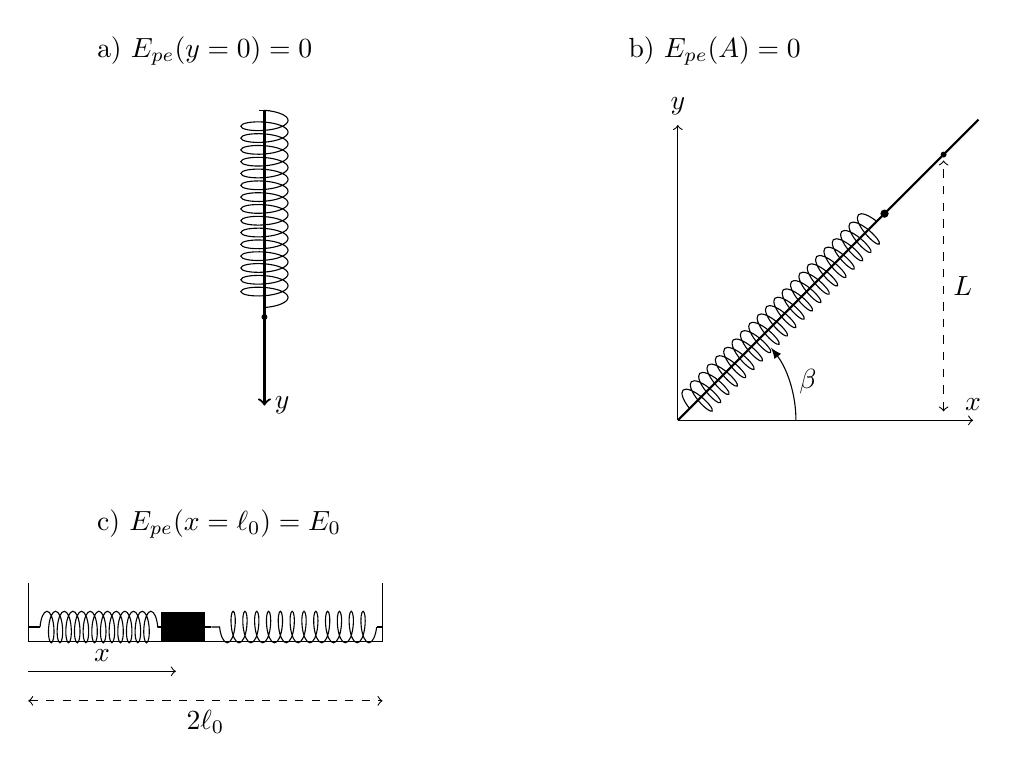
\begin{tikzpicture}[scale=.75]

\draw (-6,0) node[right]{a) $E_{pe}(y=0)=0$};
\begin{scope}[yshift = -1cm]
\draw[thick,->] (-3,0) -- (-3,-5) node[right]{$y$};
\draw (-3.1,0) -- (-2.9,0) node[right, xshift=1mm]{$\ptO$};
\draw[decoration={aspect=0.3, segment length=1.5mm, amplitude=3mm,coil},decorate] (-3,0) -- (-3,-3.5);
\fill (-3,-3.5) circle(.05) node[right, xshift=1.5mm]{$\ptM$};
\end{scope}

\begin{scope}[xshift = 2cm]
\draw (1,0) node[right]{b) $E_{pe}(A)=0$};

\draw[->] (2,-6.25) -- (7,-6.25) node[above]{$x$};
\draw[->] (2,-6.25) -- (2,-1.25) node[above]{$y$};
\draw[<->,dashed] (6.5,-6.1) -- (6.5,-1.85) node[right,midway]{$L$};
\fill (6.5,-1.75) circle(.05) node[above]{$\ptA$};
\draw[thick] (2,-6.25) -- +(45:7.2);
\draw[decoration={aspect=0.3, segment length=1.5mm, amplitude=2.25mm,coil},decorate] (2.2,-6.05) -- (5.4,-2.85);
\draw[-latex] (4,-6.25) arc(0:38:2) node[midway,right]{$\beta$};
\fill (5.5,-2.75) circle(.07) node[below right]{$\ptM$};
\draw (2,-6.25) node[below]{$\ptO$};
\end{scope}


\begin{scope}[yshift = -2cm]
\draw (-6,-6) node[right]{c) $E_{pe}(x=\ell_0)=E_0$};
\fill (-4.75,-8) rectangle (-4,-7.5);
\draw (-7,-7) -- (-7,-8) -- (-1,-8) -- (-1,-7);
\draw[decoration={aspect=0.3, segment length=1.1mm, amplitude=2mm,coil},decorate] (-6.8,-7.75) -- (-4.8,-7.75);
\draw (-7,-7.75) -- (-6.8,-7.75)
	  (-4.8,-7.75) -- (-4.75,-7.75);
\draw[decoration={aspect=0.3, segment length=1.5mm, amplitude=2mm,coil},decorate] (-1.1,-7.75) -- (-3.9,-7.75);
\draw (-4,-7.75) -- (-3.9,-7.75)
	  (-1,-7.75) -- (-1.1,-7.75);
\draw[dashed,<->] (-7,-9) -- (-1,-9) node[below,midway]{$2\ell_0$};
\draw[->] (-7,-8.5) -- (-4.5,-8.5) node[midway,above]{$x$};
\end{scope}



\end{tikzpicture}